\begin{figure*}[ht]
 \centering
 %\includegraphics[scale=1]{figures/evaluation/rate-limiting/ajil-peek.eps}
 \includegraphics[scale=1]{figures/evaluation/rate-limiting/ajil-linear.eps}
 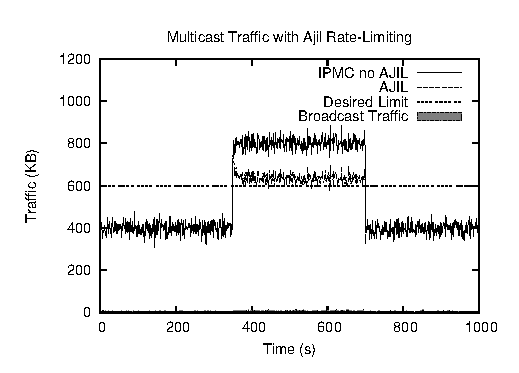
\includegraphics[scale=1]{figures/evaluation/rate-limiting/ajil-square.eps}
 \caption{Multicast traffic rate-limited by \sysname{} under different communication patterns.}
 \label{fig:rate-limiting}
\end{figure*}

In this section, we evaluate the \sysname{} protocol by simulation. The simulator uses the previously described algorithm and some simple acceptable use policies.

Our evaluation has multiple goals. We first test our protocol's rate-limiting capabilities with a couple of multicast traffic patterns. We then evaluate the effects of manipulating the protocol's parameters as part of the AUP. Additionally we test how the slowdown policy is being applied across groups and individual communication channels. Finally we test two simple administrator-defined slowdown policies and highlight their differing effects.

\subsection{Setup}
We based the setup of our nodes and multicast groups on a previously-acquired multicast trace of an IBM Websphere \cite{websphere} deployment. That trace showed an internal publish-subscribe component of Websphere using over 6,600 multicast groups averaging 10 members per group.

Our simulator generates multiple communication patterns to reflect different data center deployments. During initialization, nodes subscribe to the various multicast groups uniformly and read-in a program file dictating the number and size of messages to be sent during each epoch. This file simulates the application load. From the perspective of our protocol, during each epoch the application sends multicast requests down to the protocol which puts them down on the network as long as its current quota has not been exceeded. At the end of each epoch, nodes reevaluate their sending quota for every multicast channel on each group. We have assumed a model in which sending packets up to the current quota and then dropping the rest is acceptable.

\subsection{Rate-Limiting}
Figure ~\ref{fig:rate-limiting} shows the aggregate multicast traffic of a network with a soft rate-limit of 600 KBps. The figure depicts two communication patterns. Both networks start with traffic rates of about 400KBps. The first graph on the left shows a continuous gradual increase in raw IP Multicast traffic in the unmanaged case. When \sysname{} is used to manage multicast, the traffic increase is severely limited. The managed multcast rate does not drop below the desired limit in the first graph because \sysname{} is reactive in nature, and thus the bandwidth is adjusted in every epoch reflecting the state as it was in previous epochs.

%The first graph on the left shows a gradual increase of the communication rate to over 800KBps and then a graduate decline. This pattern arises in situations where ``flash'' multicast groups are setup dynamically to execute certain jobs and are then deleted. A gradual incline/decline is the result of inter-dependencies between the jobs being executed. So an increasing number of ``flash groups'' could be set up to process a set of jobs, and as soon as the root job has been executed all the dependencies start to finalize and terminate. We know of at least one widely deployed commercial data center application using this pattern.

The second graph on the right represents a more common case. The aggregate traffic in the network is steady at around 400KBps when suddenly an event, or a faulty process, triggers high multicast rates which push the aggregate traffic over the set limit. As soon as that event terminates the traffic rates go back to normal.

Both graphs in figure ~\ref{fig:rate-limiting} show that \sysname{} does not affect the multicast rates as long as they do not exceed the limit. Once the limit is exceeded, \sysname{} minimizes the excess. Notice that the lower peeks above the limit line in both graphs are those of rate-limited multicast. Even though the raw traffic rates exceed the limit by over 20\%, by using \sysname{} this excess is sharply reduced.

In this experiment we set the protocol parameters to: $\alpha=0.5, \beta=0.25$, and a monitor broadcast factor $c=0.01$. Notice that in both graphs the aggregate broadcast traffic used by all the monitors is reported at the bottom and is minimal in comparison to the aggregate multicast traffic in use.

\begin{figure}[t]
 \centering
 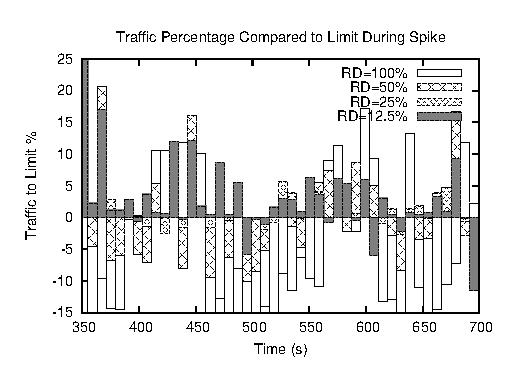
\includegraphics[scale=1]{figures/evaluation/rd/reaction-waves.eps}
 \caption{The oscillation effect in different reaction domain sizes.}
 \label{fig:varied-rd}
\end{figure}

\subsection{Reaction Domain Size}
We tested various sizes for the reaction domain trying to determine an optimal selection. We note that the effects of the size of the reaction domain are largely dependent on the slowdown policy specified by the administrator. For example, using a reaction domain encompassing all the nodes and a slowdown policy that scales back the quotas for all the senders by a fixed percentage has the effect of scaling down the entire network when the global limit is violated. On the other hand, if the administrator wishes to balance the multicast bandwidth consumption between the nodes, she might opt for choosing smaller reaction domains and implementing a slowdown policy that scales back the top senders to either a fixed upper-limit or by a fraction of their previous sending quota.

\begin{figure*}[t]
 \centering
 \includegraphics[scale=1]{figures/evaluation/staleness/excess-during.eps}
 \includegraphics[scale=1]{figures/evaluation/staleness/utility-after.eps}
 \caption{The effects of monitor staleness.}
 \label{fig:monitor-staleness}
\end{figure*}

However we observe that regardless of the slowdown policy in use, a certain pattern emerges. Since nodes rely on data of previous epochs to estimate the global traffic for subsequent epochs, it is often the case that when a group of nodes slow down in an epoch, the aggregate traffic in the subsequent epoch falls below the global limit. This can be either because of the slowdown mechanism being applied, or because other senders that were not part of the reaction domain have reduced their rates due to a reduced demand by the application. In that case, all the nodes that slowed down in the previous epoch will decide to increase their quota in the next epoch. This will result in exceeding the limit in the next epoch. This pattern of overshooting and undershooting can continue for multiple epochs. This results in an oscillatory pattern of traffic surging above or dropping below the limit.

This oscillation, however, dampens with time. This is caused by several factors: first, when nodes increase their quota after being slowed down, they do that in a multiplicative way, and the quota increase amounts to 50\% of the quota reduction implemented in the previous epoch. In addition to that, nodes that are currently applying a slowdown policy do not decrease their quota after they have increased it. This means that the multiplicative increases can not be rolled back after they have been issued. So in each epoch, the percentage by which a node in the reaction domain can speed up and slow down is monotonically decreasing. Thus this oscillatory behavior dampens with time.

However, the speed of this dampening depends on the size of the reaction domain. In large reaction domains, the oscillation is bigger in magnitude because there are more nodes that can potentially slowdown or speed up after each epoch. Figure ~\ref{fig:varied-rd} shows the oscillatory behavior of different reaction domains. In this experiment we fixed the communication pattern, and the network setup while varying the size of the reaction domain. We set the $(\alpha, \beta)$ parameters to: (1,1) which is 100\% of the nodes, and (1, 0.5), (0.5, 0.5), (0.5, 0.25) which roughly correspond to 50\%, 25\% and 12.5\% of all the nodes in a setting were the nodes are equally distributed among all the groups. Figure ~\ref{fig:varied-rd} plots the percentage of the difference between aggregate traffic rates and the imposed limit. So a value of +5\% denotes exceeding the limit by 5\%, and -5\% denotes sending 5\% below the limit. As illustrated by figure ~\ref{fig:varied-rd}, smaller reaction domains experience smaller-magnitude oscillation as expected.




\subsection{Monitor Staleness}

As explained previously, nodes rely on the monitor component of the protocol to gather data about the sending patterns of other nodes and other groups in the system. Nodes then use that collected information to make local decisions on whether to invoke the reactor and apply the slowdown policy or not. Monitors use a broadcast channel and probabilistically publish the traffic rates of their nodes. In this experiment we manipulated the monitor broadcast frequency ($c$) to measure its effect on the responsiveness of the protocol. A low broadcast frequency implies a lower probability for a particular monitor to publish its most recent information, which also implies that nodes often have to rely on old stale data when reevaluating the sending quota between epochs. This staleness implies a slower reaction to a limit violation, and a slower speedup after the violation has been removed.

\begin{figure*}[t]
 \centering
 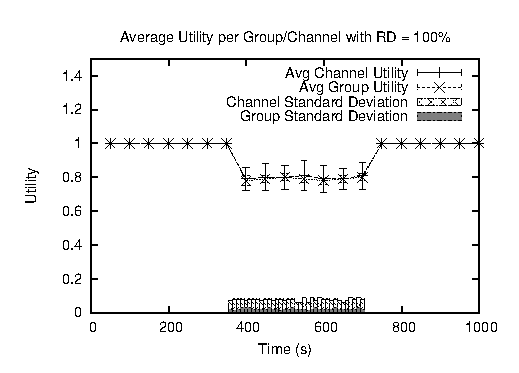
\includegraphics[scale=1]{figures/evaluation/fairness/utility-rd1.eps}
 \includegraphics[scale=1]{figures/evaluation/fairness/utility-rd.125.eps}
 \caption{The average ratio of the allotted quota to the requested quota of each group and channel.}
 \label{fig:utility}
\end{figure*}

Figure ~\ref{fig:monitor-staleness} shows the affect of the broadcast frequency $c$ on the responsiveness of the protocol. We used the square wave traffic pattern as shown in the right graph of figure ~\ref{fig:rate-limiting} where the limit is being exceeded during the time interval [350, 700]. We measured the responsiveness of the system under two broadcast frequencies: $c=0.01$ which has been used for the rest of the experiments thus far, and a smaller $c=0.001$. The first graph on the left in figure ~\ref{fig:monitor-staleness} shows the percentage by which \sysname{} overshoots the limit during the time the limit is being exceeded. As expected, with a smaller broadcast frequency, nodes are less aware of the changes in the sending patterns of other nodes, and thus their bandwidth quotas have not been limited to avoid the excess. This results in the protocol overshooting beyond the limit by a larger fraction than that experienced by the larger $c$ value.

The broadcast frequency also affects the responsiveness of the protocol in recovering from a limit violation. The second part on the right of figure ~\ref{fig:monitor-staleness} shows how quickly the protocol recovers from the limit violation. The graph shows the total allotted quota as a percentage of the requested quota after the limit violation has ended. In an optimal case, the utility should be 100\% immediately after time $t=700$, since that is when the spike ends as shown in figure ~\ref{fig:rate-limiting}. As expected, we see that a higher broadcast frequency results in a faster recovery from a limit violation, because nodes are more aware of the reduced sending rates of other nodes and thus expand their own quotas.

\subsection{Fairness and Utility}

We achieved rate-limiting by slowing down a subset of the senders in the system. However, in the worst case scenario this could result in a subset of the senders being completely denied multicast access while other nodes receive the full bandwidth quota that they ask for. We define \textit{utility} as the percentage of the requested bandwidth that is ratified by the sending quota of a node or group. We get a sense of the 'fairness' of the protocol by analyzing the variance of the utilities on each multicast group: a high variance implies an uneven distribution of utilities among the nodes. We can also measure the utility of each channel (sender on a group). Intuitively, the fairness of the protocol depends on the administrator's policy and the protocol parameters.

Figure ~\ref{fig:utility} shows the utility per channel and per group for the same network under two different policies. In both cases the slowdown policy has been set to slowdown the nodes in the reaction domain by a percentage that is proportional to the fraction of traffic being sent in excess above the global rate limit. However, in the first graph on the left the reaction domain has been set to include all the nodes and all the senders (i.e. the entire network scales back when the limit is violated). Meanwhile, the second graph on the left uses the 12.5\% reaction domain ($\alpha=0.5, \beta=0.25$) that we have seen before.

As expected, the variance of the group utility is much lower with the reaction domain is larger because more groups are being scaled back. In both cases the variance of the channels utility is larger than the variance of the groups utility. This is because the uniform distribution of nodes to groups results in having the bandwidth demands for groups be very comparable. However, each channel represents the multicast demands of a single node on a single group. So channels are much more varied by definition. This means that when channels with low demands are slowed down their nodes will increase and regain their quotas quickly because they do not contribute much to the overall aggregate traffic and will thus find the capacity to increase their quotas. This means that low demand channels can achieve 100\% utility much easier than large demand channels. This heterogeneity between the channels demands results in a more varied utility for them, which explains the higher variance we see in figure ~\ref{fig:utility} for channels when compared to groups.


\subsection{Policy}
In the experiments we ran so far, we have used a single slowdown policy. The slowdown mechanism involved reducing the quota of all the nodes in the reaction domain by the same fraction as the excess in multicast traffic above the aggregate limit. However, as eluded to before, the choice of policy has direct impact on the performance of the protocol.

\begin{figure*}[t]
 \centering
 \includegraphics{figures/evaluation/policy/ajil-policy1.eps}
 \includegraphics{figures/evaluation/policy/channels-utility.eps}
 \includegraphics{figures/evaluation/policy/ajil-policy2.eps}
 \includegraphics{figures/evaluation/policy/groups-utility.eps}
 \caption{The top left part shows a naive slowdown policy resulting in unstable traffic when the multicast demand exceeds the global limit. The bottom left part shows a more stable slowdown policy producing a more stable traffic pattern. The right side shows the effects of the two policies on group and channel utilities.}
 \label{fig:policy}
\end{figure*}

In this experiment we implemented another slowdown policy with a strict and naive slowdown mechanism dictating that nodes in the reaction domain set their quotas to 0 in the first epoch in which they are in the reaction domain, and then multiplicatively increase their quota (by multiplicatively decreasing the slowdown amount by 50\% if possible). As figure ~\ref{fig:policy} shows, although this policy quickly reduces the violating traffic, it does not result in fairly distributed group and channel utilities.

The top left part of figure ~\ref{fig:policy} shows the aggregate traffic as a result of running the naive policy (\#1) as compared with running our old, fraction-based, policy (\#2) in the bottom left. Although the naive policy cuts excess traffic more quickly than the old policy, it results in extreme fluctuation of traffic rates near the limit. This happens because as soon as the global traffic reaches the limit, a bunch of nodes stop sending immediately causing a quick dip in the aggregate traffic. Following that, the nodes start sending again and the pattern repeats.

The right side of figure ~\ref{fig:policy} shows the difference in channel and group utilities between the two policies. On the top we see that the per-channel utilities are much more variant under the naive policy. This follows intuition because channels are repeatedly being closed (quota set to 0) and then reopened. A similar effect is seen for the group utilities at the bottom right part of the figure.
